\documentclass{article}
\usepackage{tikz}
\usetikzlibrary{bayesnet}

\begin{document}

\title{Graphical Representation for Exploratory Analysis}
\author{}
\date{}
\maketitle

The following diagram illustrates the hypothesized relationships between the language condition (Italian vs. English) and the illusion of causality via the four mediators: task difficulty, emotional distancing, prior knowledge, and the weaker associative memory strength.
\vspace{1cm}

\centering
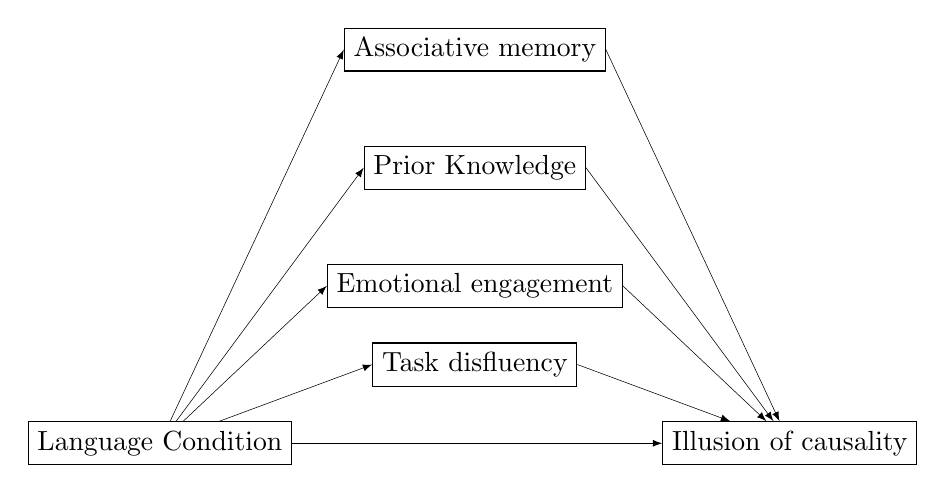
\begin{tikzpicture}[scale=1]

    \node[draw] (AA) at (0,1) {Task disfluency};
    \node[draw] (G) at (0,2) {Emotional engagement};
    \node[draw] (H) at (0,3.5) {Prior Knowledge};
    \node[draw] (I) at (0,5) {Associative memory};

    \node[draw] (L) at (4,0) {Illusion of causality};
    \draw [<-, very thin, >=latex] (L)--(G.east) ;
    \draw [<-, very thin, >=latex] (L)--(H.east) ;
    \draw [<-, very thin, >=latex] (L)--(I.east) ;
    \draw [<-, very thin, >=latex] (L)--(AA.east) ;

    \node[draw] (Z) at (-4,0) {Language Condition};
    \draw [->, very thin, >=latex] (Z)--(G.west) ;
    \draw [->, very thin, >=latex] (Z)--(H.west);
    \draw [->, very thin, >=latex] (Z)--(I.west);
    \draw [->, very thin, >=latex] (Z)--(AA.west);
    \draw [->, very thin, >=latex] (Z)--(L);

\end{tikzpicture}

\end{document}
